%%% Copyright (C) 2015-2024 Vincent Goulet
%%%
%%% Ce fichier fait partie du projet
%%% «Rédaction avec LaTeX»
%%% https://gitlab.com/vigou3/formation-latex-ul
%%%
%%% Cette création est mise à disposition sous licence
%%% Attribution-Partage dans les mêmes conditions 4.0
%%% International de Creative Commons.
%%% https://creativecommons.org/licenses/by-sa/4.0/

\section{Principes de base}

\begin{frame}[fragile=singleslide]
  \frametitle{Séparation du contenu et de l'apparence}

  L'apparence du document est prise en charge par {\LaTeX} et
  il est généralement préférable de ne pas la modifier.

  \begin{itemize}
  \item On se concentre sur le \alert{contenu} et la \alert{structure} du
    document
  \item On indique la sémantique du texte et non son apparence
    \begin{demo}
      \begin{minipage}{0.45\linewidth}
\begin{lstlisting}
\textbf{\large Titre}
\end{lstlisting}
      \end{minipage}
      \hfill \faArrowRight \hfill
      \begin{minipage}{0.45\linewidth}
\begin{lstlisting}
\section{Titre}
\end{lstlisting}
      \end{minipage}
    \end{demo}
  \end{itemize}
\end{frame}

\begin{frame}[fragile]
  \frametitle{Règles de saisie}

  \begin{enumerate}[<+| only@+>]
  \item Mots séparés par une ou plusieurs \alert{espaces}
\begin{demo}
    \begin{texample}
\begin{lstlisting}
Les espaces délimitent les
mots. Leur nombre n'a pas
d'importance.
\end{lstlisting}
      \producing
      Les espaces délimitent les
      mots. Leur nombre n'a pas
      d'importance.
    \end{texample}
    \begin{texample}
\begin{lstlisting}[showstringspaces=true]
Les  espaces   délimitent
les                 mots.
Leur    nombre  n'a pas
d'importance.
\end{lstlisting}
      \producing
      Les  espaces   délimitent
      les                 mots.
      Leur    nombre  n'a pas
      d'importance.
    \end{texample}
  \end{demo}
  \item Paragraphes séparés par une ou plusieurs \alert{lignes
      blanches}
    \begin{demo}
      \begin{texample}
\begin{lstlisting}
Les lignes blanches
délimitent les paragraphes.

Une ou plusieurs, ça ne fait
aucune différence!
\end{lstlisting}
      \producing
Les lignes blanches
délimitent les
paragraphes.

Une ou plusieurs, ça ne fait aucune différence!
      \end{texample}
      \begin{texample}
\begin{lstlisting}
Les lignes blanches
délimitent les paragraphes.


Une ou plusieurs, ça ne fait
aucune différence!
\end{lstlisting}
      \producing
        Les lignes blanches  délimitent
        les paragraphes.



        Une ou plusieurs, ça ne fait aucune différence!
      \end{texample}
    \end{demo}
  \item Utilisation de \alert{commandes} pour indiquer la structure du
    texte
    \begin{demo}
      \begin{texample}
\begin{lstlisting}
Les commandes sont visibles
dans le \textbf{texte},
mais évidemment pas dans le
\emph{document} fini.
\end{lstlisting}
        \producing
        Les commandes sont visibles
        dans le \textbf{texte},
        mais évidemment pas dans le
        \emph{document} fini.
      \end{texample}
    \end{demo}
  \end{enumerate}
\end{frame}

\begin{frame}[fragile=singleslide]
  \frametitle{Caractères réservés}

  \begin{itemize}
  \item Caractères réservés par {\TeX}:
    \begin{quote}
      \code{\#~\$~\&~\string~~\_~\string^~\%~\{~\}}
    \end{quote}
  \item Pour les utiliser, précéder par «\bs»
    \begin{demo}
      \begin{texample}
\begin{lstlisting}
L'augmentation de 2~\$
représente une hausse
de 5~\%.
\end{lstlisting}
        \producing
        L'augmentation de 2~\$ représente une
        hausse de 5~\%.
      \end{texample}
    \end{demo}
  \end{itemize}
\end{frame}

\begin{frame}[fragile=singleslide]
  \frametitle{Structure d'un document {\LaTeX}}

  Un fichier source {\LaTeX} est toujours composé de deux parties.

  \begin{minipage}{0.2\linewidth}
    \begin{minipage}{\linewidth}
      \hfill préambule \quad
      \rule[-10mm]{1pt}{21mm}
    \end{minipage} \\[5mm]
    \begin{minipage}{\linewidth}
      \hfill corps \quad
      \rule[-15mm]{1pt}{30mm}
    \end{minipage}
  \end{minipage}
  \hfill
  \begin{minipage}{0.75\linewidth}
\begin{lstlisting}[emph={documentclass,begin,end,document}]
\documentclass[11pt,french]{article}
  \usepackage{babel}
  \usepackage[autolanguage]{numprint}
  \usepackage[utf8]{inputenc}
  \usepackage[T1]{fontenc}

\begin{document}

Lorem ipsum dolor sit amet, consectetur
adipiscing elit. Donec quam nulla, bibendum
vitae ipsum vel, fermentum pellentesque orci.

\end{document}
\end{lstlisting}
  \end{minipage}
\end{frame}

\begin{frame}[fragile=singleslide]
  \frametitle{Commandes}
  \begin{itemize}
  \item Débutent toujours par «\bs»
  \item Exemples de syntaxe
\begin{lstlisting}
\LaTeX                   % aucun argument
\emph{toujours}          % un argument obligatoire
\section*{Introduction}  % effet modifié
\rule[6pt]{5mm}{2pt}     % un argument optionnel, deux obligatoires
\end{lstlisting}
   \item Commande sans argument: le nom se termine par tout
    caractère qui n'est \alert{pas une lettre} (y compris l'espace!)
  \item Portée d'une commande limitée à la zone entre \code{\{~\}}
  \end{itemize}
\end{frame}

\begin{frame}[fragile=singleslide]
  \frametitle{Environnements}
  \begin{itemize}
  \item Délimités par
\begin{lstlisting}
\begin`\marg{environnement}'
   ...
\end`\marg{environnement}'
    \end{lstlisting}
  \item Contenu de l'environnement traité différemment du reste du texte
  \item Changements s'appliquent uniquement à l'intérieur de
    l'environnement
  \end{itemize}
\end{frame}

\begin{frame}[fragile]
  \frametitle{{\LaTeX} en français}

  Approche moderne \alert{vivement recommandée}: enregistrer le code
  source en \link{https://fr.wikipedia.org/wiki/UTF-8}{UTF-8} et
  compiler avec {\XeLaTeX}.

  Il faut ensuite charger quelques paquetages pour franciser \LaTeX.
  \begin{itemize}
  \item \pkg{babel}: traduction des mots-clés prédéfinis,
    typographie française, coupure de mots, document multilingue
  \item \pkg{icomma}: virgule comme séparateur décimal
  \item \pkg{numprint}: espace comme séparateur des milliers
  \end{itemize}
\end{frame}

\begin{exercice}
  Modifier le fichier \fichier{exercice-commandes.tex} afin de
  produire le texte ci-dessous.

  \bigskip
  \centering
  \fbox{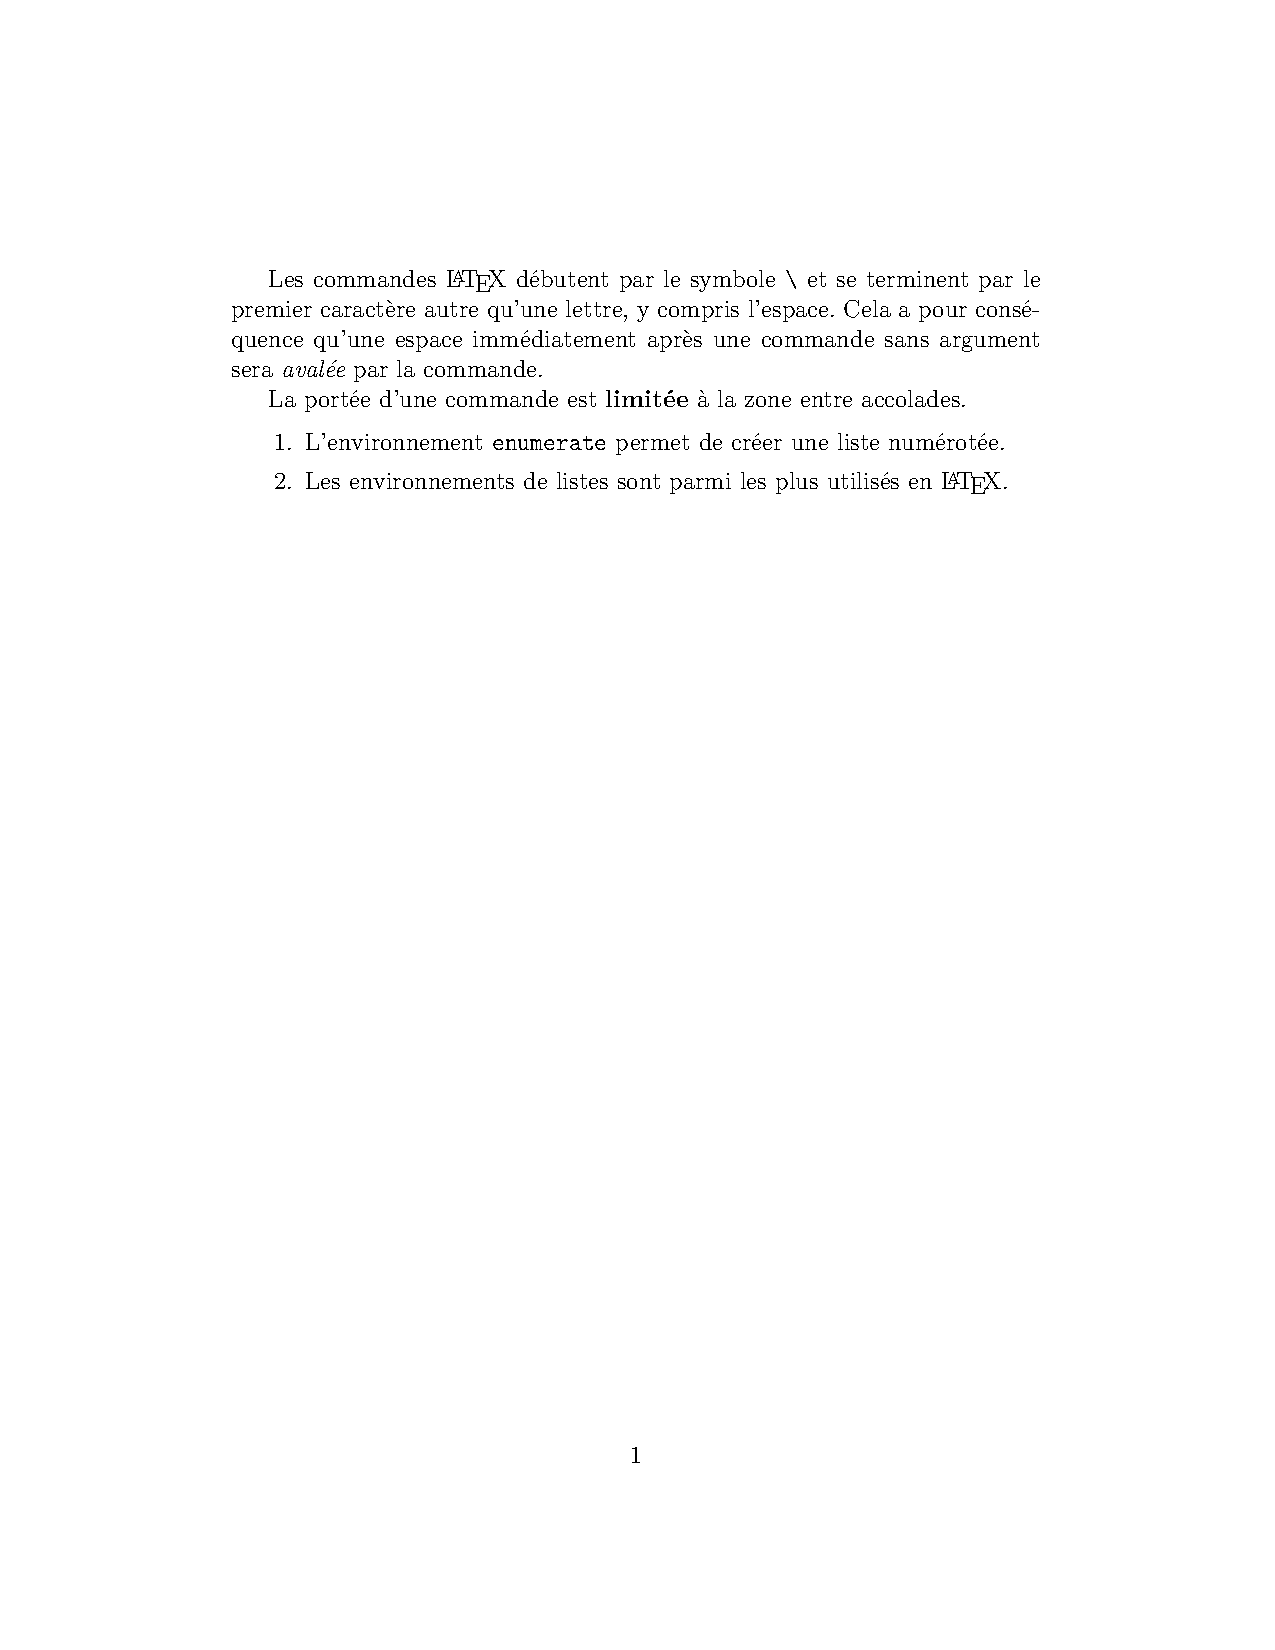
\includegraphics[viewport=108 551 502 665,%
    clip=true,width=0.9\linewidth]{auxdoc/exercice-commandes-solution}}
\end{exercice}

%%% Local Variables:
%%% TeX-master: "formation-latex-ul-diapos"
%%% TeX-engine: xetex
%%% coding: utf-8
%%% End:
